\subsection{Dataset}
Insect pests evolve and change their visuals during all their lifetime depending on the species and category. Collecting and classifying pest images becomes more difficult due to these reasons.

\begin{center}
\begin{figure}[htb]
    \centering
    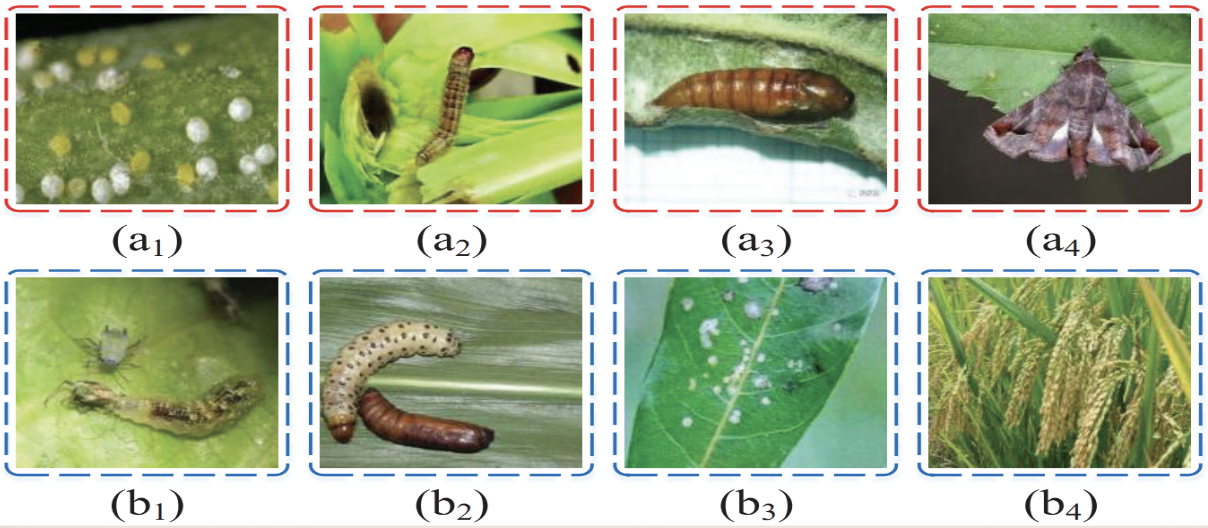
\includegraphics[scale=.7]{figures/ip102.png}\\
    \caption{IP102 Sample Images of different growthstage and multiple samples \cite{wu2019ip102}}
    \label{fig:ip102}
\end{figure}
\end{center}
Hence we have used a public dataset named IP102. It is a large dataset containing more than 75,000 images belonging to 102 classes. Some sample images from the dataset are shown in fig \ref{fig:ip102}. This dataset is mainly devided into two categories- field crops and Economic crops. Field crops consist of five super classes- Rice, Corn, Wheat, Beet, Alfalfa. Economic crops consist of three super classes- Vitis, Citrus, Mango.

\newpage
Hence we have used a public dataset named IP102. It is a large dataset containing more than 75,000 images belonging to 102 classes. Some sample images from the dataset are shown in fig \ref{fig:ip102}. This dataset is mainly devided into two categories- field crops and Economic crops. Field crops consist of five super classes- Rice, Corn, Wheat, Beet, Alfalfa. Economic crops consist of three super classes- Vitis, Citrus, Mango.
\newpage
Hence we have used a public dataset named IP102. It is a large dataset containing more than 75,000 images belonging to 102 classes. Some sample images from the dataset are shown in fig \ref{fig:ip102}. This dataset is mainly devided into two categories- field crops and Economic crops. Field crops consist of five super classes- Rice, Corn, Wheat, Beet, Alfalfa. Economic crops consist of three super classes- Vitis, Citrus, Mango.
\newpage

\begin{figure}
    \centering
    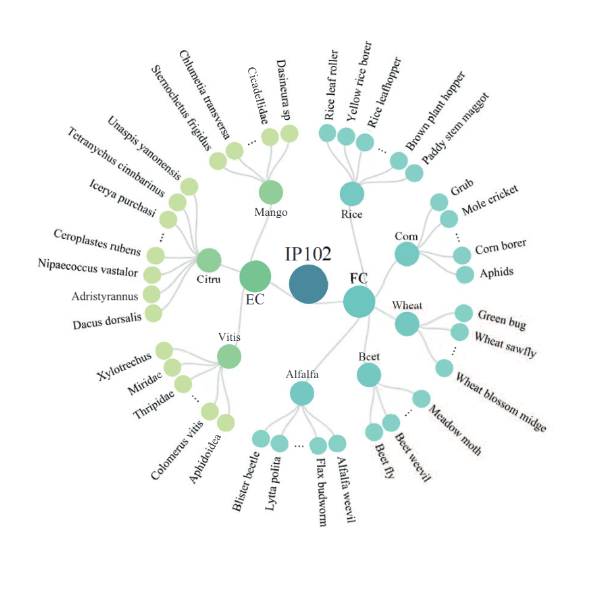
\includegraphics[scale=1.4]{figures/ip102map.png}
    \caption{ Taxonomy of the IP102 dataset \cite{wu2019ip102}}
    \label{fig:my_label}
\end{figure}


\begin{center}
    \begin{center}
\centering
\begin{table}[!htbp]
\begin{tabular}{|c|c|c|c|c|c|p{3cm}|p{2cm}|}
\hline
\multicolumn{2}{|l|}{\textbf{Superclass}} & \textbf{Class} & \textbf{Train} & \textbf{Val} & \textbf{Test} & \textbf{Total sample / superclass} & \textbf{IR*}\\
\hline
\multirow{5}{3em}{RC*} & Rice & 14 & 5,043 & 843 & 2,531 & 8,417 & 6.4 \\\cline{2-8}
& Corn & 13 & 8,404 & 1,399 & 4,212 & 14,015 & 27.9 \\\cline{2-8}
& Wheat & 9 & 2,048 & 340 & 1,030 & 3,418 & 5.3 \\\cline{2-8}
& Beet & 8 & 2,649 & 441 & 1,330 & 4,420 & 15.4\\\cline{2-8}
& Alfalfa & 13 & 6,230 & 1,037 & 3,123 & 10,390 & 10.7\\\cline{2-8}
\hline
\multirow{3}{3em}{EC*} & Vitis & 16 & 10,525 & 1,752 & 5,274 & 17,55 & 74.8\\\cline{2-8}
& Citrus & 19 & 4,356 & 725 & 2,192 & 7,273 & 17.6 \\\cline{2-8}
& Mango & 10 & 5,840 & 971 & 2,927 & 9,738 & 61.7\\\cline{2-8}
\hline
\multirow{2}{3em}{IP102} & FC & 57 & 24,374 & 4,060 & 12,226 & 40,660 & 39.4\\\cline{2-8}
& EC & 45 & 20,721 & 3,448 & 10,393 & 34,562 & 80.8\\\cline{2-8}
\hline
Total & IP102 & 102 & 45,095 & 7,508 & 22,619 & 75,222 & 80.8\\\cline{2-8}
\hline
\end{tabular}
\caption{IP102 Dataset\\ FC = Field crops,    EC = Economicalcrops, IR = Imbalance Ratio}
\label{table_ip102}
\end{table}
\end{center}
\end{center}

\vspace{300px}

\newpage

\subsection{Data preparation, Pre-processing and Training  procedure}
Millions of parameters are worked on a neural network system. For better generalization capability it is essential to perform data augmentation in the dataset. All the images of the dataset are resized to \(224 * 224 * 3\) and RGB format for performance betterment of the system. The data are kept with maintaining proportion so that a good learning capacity can be achieved. Different augmentation like horizontal flipping, vertical flipping, 10° rotation and slant angle (0.2) for sheer transformation is done to both training and validation data to make up for the lack of data availability. Different types of inputs are being used to validate the model. For that, the validation data portion is also augmented. Both synthetically modified data and validated augmented data are required for the learning of the models. The images are normalized by dividing the images using RGB channel mean and calculating standard deviation of the images in the ImageNet1K dataset ([0.485, 0.456, 0.406] and [0.229, 0.224, 0.225]) so that uniform data distribution can be ensured. This also ensures better convergence of the model during the training of the neural network. Dataset splitting for train, validation, and testing has been maintained with a 6:1:3 ratio. For training all images are normalized to the . For all models, the final linear classification layer is replaced with a new layer with as many output nodes as there are classes to classify the dataset, and model parameters are optimized so that the categorical cross-entropy loss function is minimized.  If we consider the probabilities of the events from P and Q, then cross-entropy can be calculated as-
\begin{equation}
    H(P, Q) = -sum(x)\text{ in X } P(x) * \log(Q(x))
\end{equation}


\subsection{Experimental Setup}
Colab and Kaggle Notebooks were used to generate a python environment with Pytorch and other python libraries to carry out the experiment of the proposed method. An Intel Xeon CPU @ 2.00 GHz, thirteen(13) GB Ram and a  Tesla P100 16GB VRAM as GPU were used to conduct most of the experiments. On the other hand we also used high config Intel Core I9 pc with 24 gb nvdia rtx 3080 for some heavy computation task like segmentation.

For all the classes, the sample images were split into a 6:3:1 ration for training, validation and testing. Batch size 32 was selected for mini batch gradient descent. Early stopping was used which help to reduce overfitting problem and improve generalization of the model. Each pretrained model was set to train for at least 25 epoch with early stopping. In our method, a change of \(10^{-4}\) is considered great. Otherwise it is considered a not improving epoch. The setting was made to stop training early if the training completes ten consecutive non imroving epochs. On average most of the models were able to converge after 20 epochs but two of them got early convergence after 10 epochs. For optimization Adam optimizer was used as it is usually recommended for classification tasks. Adam optimizer has faster computation time and fewer parameters tuning.

Since it is a multiclass classification task, cross entropy loss was used to calculate the loss.Firstly, the learning rate was set to 0.001 and after every seven non improving epochs, the learning rate was set to decrease by a factor of 0.1 to assist the model for finding a set of globally optimal weights that improve generalization. In the experiment, pretrained models were initialized using ImageNet dataset’s weight. Model checkpoints were used to save the model with the best validation accuracy so that the training can be continued later from the point it was stopped.

\begin{figure}
    \centering
    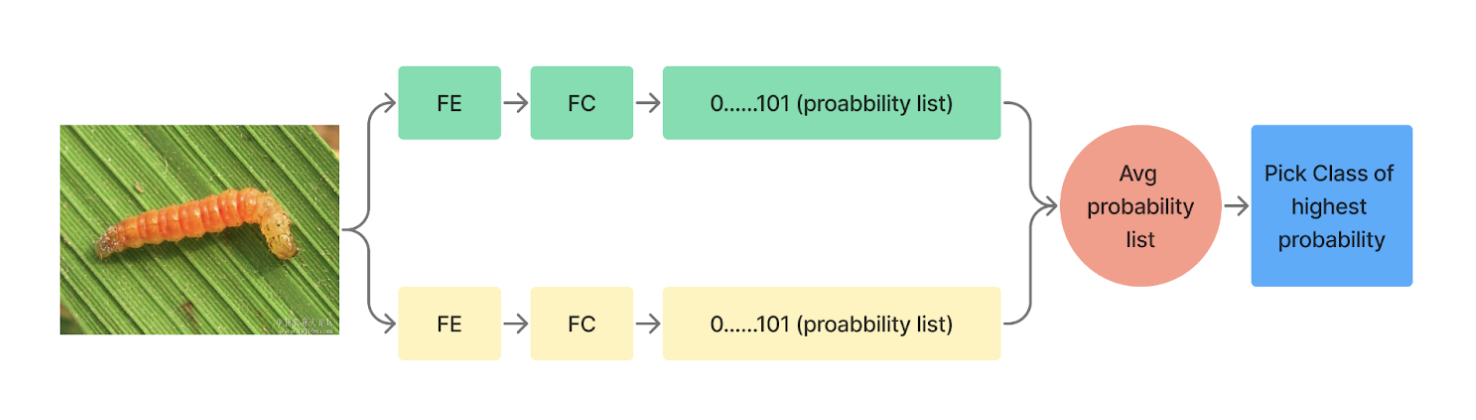
\includegraphics[scale=0.5]{figures/ensemble_model.png}
    \caption{Ensemble Technique}
    \label{fig:my_label}
\end{figure}

\subsection{Experiment Methods}
\subsubsection{Convolutional Neural Networks}
Convolutional Neural Networks \cite{lecun1998gradient} (CNNs) have emerged as a prominent and extensively employed deep learning methodology within the domains of computer vision and image processing. CNNs have brought about a paradigm shift in a transformative era in handling image-related tasks, such as image classification, object detection, and image segmentation. A fundamental strength inherent in CNNs is their innate capacity to automatically acquire and extract hierarchical features from unprocessed input data. By effectively utilizing convolutional layers, pooling operations, and non-linear activation functions, CNNs adeptly capture spatial representation and meticulously preserve vital structural information embedded within images. The multi-layer architecture of CNNs enables them to learn complex patterns and representations, making them highly suitable for tasks involving large-scale image datasets. As a result, CNNs have achieved remarkable performance improvements in image recognition tasks, surpassing traditional machine learning methods and setting new benchmarks

\subsubsection{Transfer learning and Fine Tuning}
Transfer learning is where there are pretrained models which are previously trained on a big dataset and then the knowledge is transferred into the new desired dataset using fine tuning. Transfer learning \cite{alzubaidi2021review} leverages the idea that knowledge acquired from solving one task can be beneficial for solving a related but different task. Instead of training a model from scratch, transfer learning starts with a pre-trained model that has been trained on a large-scale dataset, typically on a source task or domain. The knowledge captured in the pre-trained model's parameters, also known as weights, can be transferred and utilized to enhance the learning process for the target task or domain utilizing fine tuning on the smaller dataset \cite{feng2012boosting}. In fine tuning the last few layers are trained again for the new dataset but not the whole architecture. It saves time and computational effort as well. It’s been very effective on the classification task. So we firstly tried different pretrained models such as ResNet, EfficientNet and so on. The last fully connected layer was changed to the class number for IP102 which is 102. Then the model was trained on the IP102 dataset. 

\begin{sidewaysfigure}
    \centering
    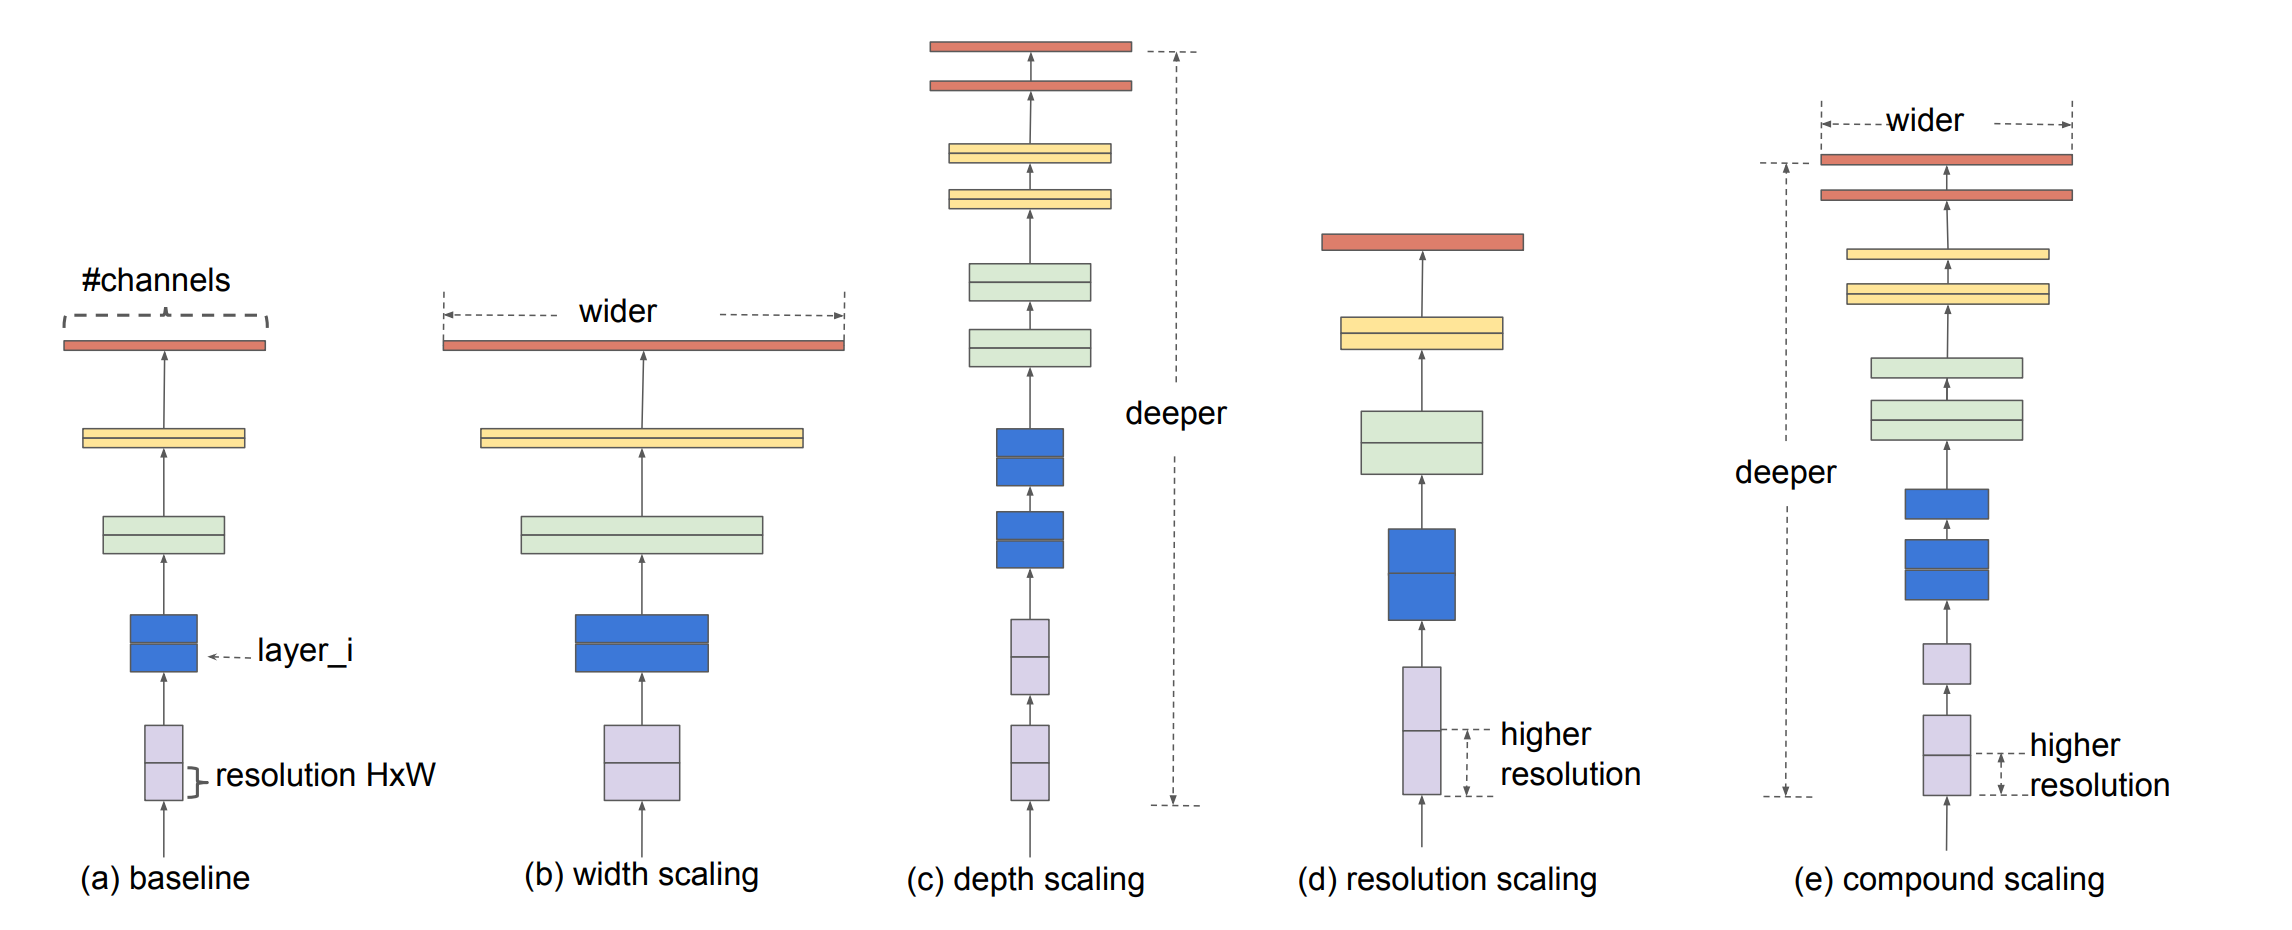
\includegraphics[scale=0.65]{figures/efficientnetArchitecture.png}
    \caption{Model Scalling of Efficient Net \cite{tan2021efficientnetv2}}
    \label{fig:my_label}
\end{sidewaysfigure}

\paragraph{Pretrained Models}
\begin{itemize}
    \item \textbf{EfficientNetV2:}
        EfficientNets \cite{tan2021efficientnetv2} are a series of CNNs that have achieved excellent results on the ImageNet \cite{krizhevsky2017imagenet} dataset. They are designed using a method called compound scaling, which involves adjusting the width, depth, and resolution of the model. The optimal values for these factors are determined using a technique called Neural Architecture Search, which aims to minimize floating-point operations number (FLOPS) required. A newer version of EfficientNets called  EfficientNetV2 \cite{tan2021efficientnetv2} has been developed, which is smaller and faster for classification tasks. It uses a different type of block called Fused-MBConv, which includes a standard convolution with 3x3 filters rather than a depthwise convolution. To the best of the authors' knowledge, there has not been any previous work on transfer learning using the EfficientNetV2 model. The authors have conducted their own experiments with transfer learning on EfficientNetV2 and found that it performs very well for classifying images as normal or abnormal.
        In this report, the ConvNeXt-L model was trained by using its default configuration . It was pretrained with the ImageNet21K dataset and has 235M parameters.
    \item \textbf{ConvNeXt:}
        ConvNeXt is a deep learning framework used for semantic segmentation and object detection.
        The attentional mechanisms are absent.
        It makes advantage of transformer networks by "modernizing" the ResNet network (ResNeXt) \cite{he2015deep}
        ResNeXt is employed rather than ResNet, despite ConvNeXt's resemblance to the Swin Transformer \cite{liu2021swin} model.
        Transformer networks make use of advances in the ConvNeXt block (e.g. AdamW optimizer).
        Figure \ref{fig:convnext} illustrates the ConvNeXt block, which includes the convolution layer, Linear Normalization with Gaussian Error Linear Unit (GELU).
    \item \textbf{Vision Transformer (ViT):}
        In the field of deep learning, attention mechanisms are a recent development that are particularly useful for natural language processing tasks. The ViT model was the first to utilize this technique in image segmentation. It works by dividing the image into smaller pieces and encoding them with position values, which are then passed to the transformer decoder for classification. By using attention mechanisms, the ViT model is able to better understand and analyze images for accurate segmentation and classification.
        \begin{figure}
            \centering
            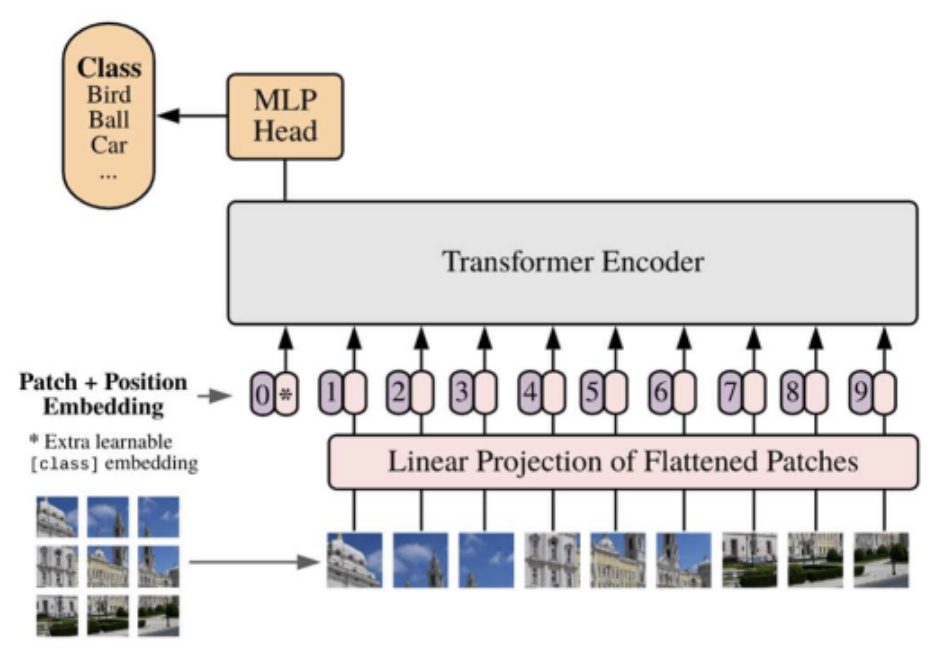
\includegraphics[scale=.7]{figures/vit.png}
            \caption{Encoder Model of ViT Network \cite{peng2022cnn}}
            \label{fig:vit}
        \end{figure}
        
        \begin{figure}[htb]
            \centering
            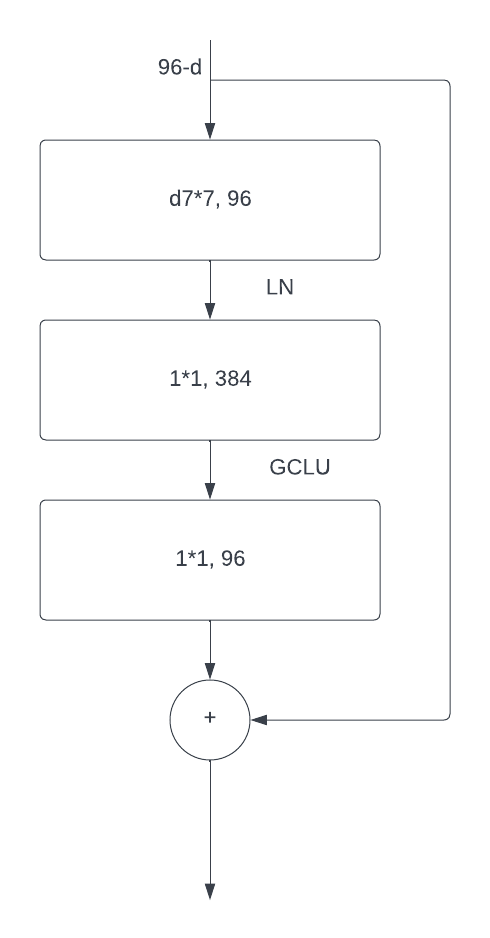
\includegraphics[scale=.7]{figures/convnext.png}
            \caption{ConvNext Block \cite{peng2022cnn}}
            \label{fig:convnext}
        \end{figure}
        Figure \ref{fig:vit} illustrates the encoder model of the vision transformer (ViT), which includes k self-attention mechanisms (also known as multihead self-attention). These mechanisms are calculated where the query matrix, key matrix, and value matrix are used to determine the attention given to each element. The multi-headed self-attention mechanism, shown in Equation 3, is made up of multiple self-attention operations and was pre-trained with ImageNet21K. In the ViT architecture, these mechanisms are used to analyze and understand the input image in order to perform accurate segmentation and classification.


\end{itemize}

\subsubsection{Attention Mechanism}
After examining the results of different pretrained models in the datasets of IP102, it is observed that the dataset is a difficult one as it has images with complex background, wild images and even sketches of pests as well. Hence the dataset gives the pretrained model a hard time to learn properly. As a result the accuracy obtained is in the range of 70~76\% which is not that satisfactory for a classification task. so we figured out that the model was not really giving attention to the portion of the images where it should give as the insects take only a small portion of the whole image. so after we implemented the idea of the literature \cite{ung2021efficient}. They presented different cnn models in their work with some attention mechanism like RAN, feature pyramid(FAN) and ensemble them to get a better result on IP102.

\paragraph{Residual Networks:}
Residual networks or ResNet \cite{he2015deep} was proposed by He et al. in 2015. This is a network architecture that utilizes skip connections, or shortcut pathways, between layers. These skip connections allow the gradient to flow back to the input more easily, which helps prevent the vanishing gradient problem that can occur when training deep neural networks. This allows the network's weights to be updated more effectively. Residual networks are made up of residual blocks that can be stacked to create very deep neural networks, potentially with over 1000 layers, depending on the specific problem being addressed. These networks are depicted in figure \ref{fig:residual_block}.

\begin{figure}[!htbp]
    \centering
    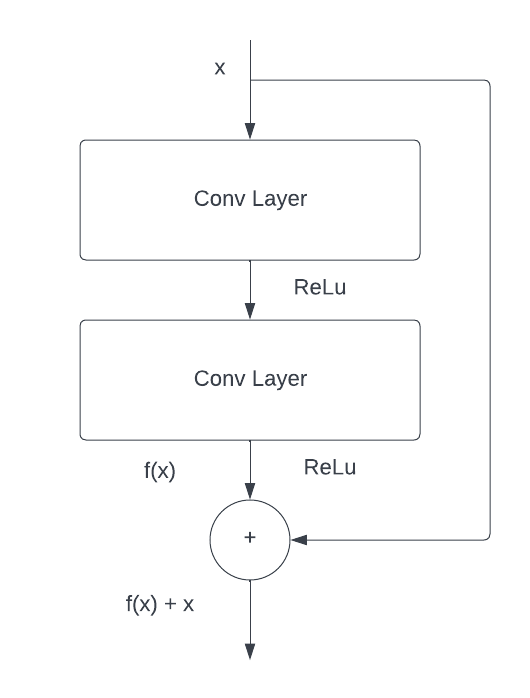
\includegraphics[scale=0.65]{figures/residual_block.png}
    \caption{Structure of a residual block in residual networks \cite{ung2021efficient}}
    \label{fig:residual_block}
\end{figure}

\paragraph{Residual Attention Networks (RAN):}

\begin{sidewaysfigure}
    \centering
    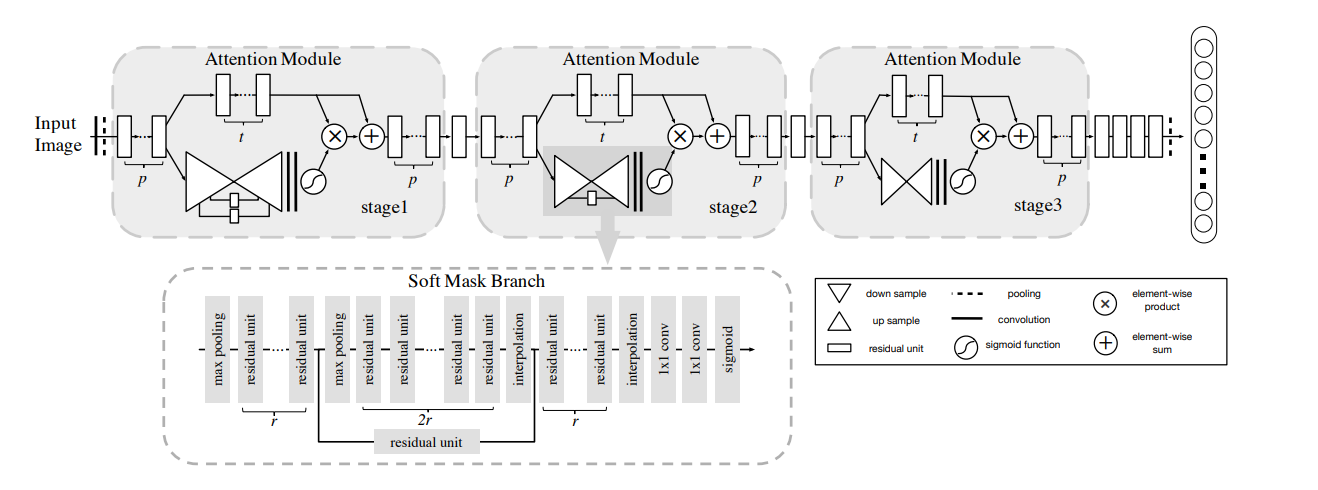
\includegraphics[scale=0.5]{figures/RAN.png}
    \caption{Residual Attention Network \cite{wang2017residual}}
    \label{fig:my_label}
\end{sidewaysfigure}

Wang et al. \cite{wang2017residual} introduced a method called (RAN) that utilizes attention mechanisms within convolutional neural networks (CNNs) to identify important areas of an image for classification. The Residual Attention Network is designed by layering numerous Attention Modules. Each of these modules comprises two parts: the mask branch and the trunk branch. The trunk branch handles feature processing and can integrate various network structures, such as pre-activation Residual Unit, ResNeXt, and Inception, used as the fundamental unit of the Residual Attention Network.The mask branch, on the other hand, uses a bottom-up top-down structure to create a mask of the same size, M(x), that softly weights output features from the trunk branch, T(x). This mask functions as control gates for the trunk branch neurons, similar to the Highway Network. The attention mask not only acts as a feature selector but also guides gradient updates during backpropagation, enhancing the module's robustness to noisy labels. A unique aspect of the Residual Attention Network is that each trunk branch within an Attention Module has its own mask branch, which learns attention specifically for its features. This enables more efficient refinement and processing of complex images. These networks are composed of multiple attention based modules that can generate attention-based features to guide the learning process, which results improved performance compared to previous methods.
\begin{figure}[!htbp]
    \centering
    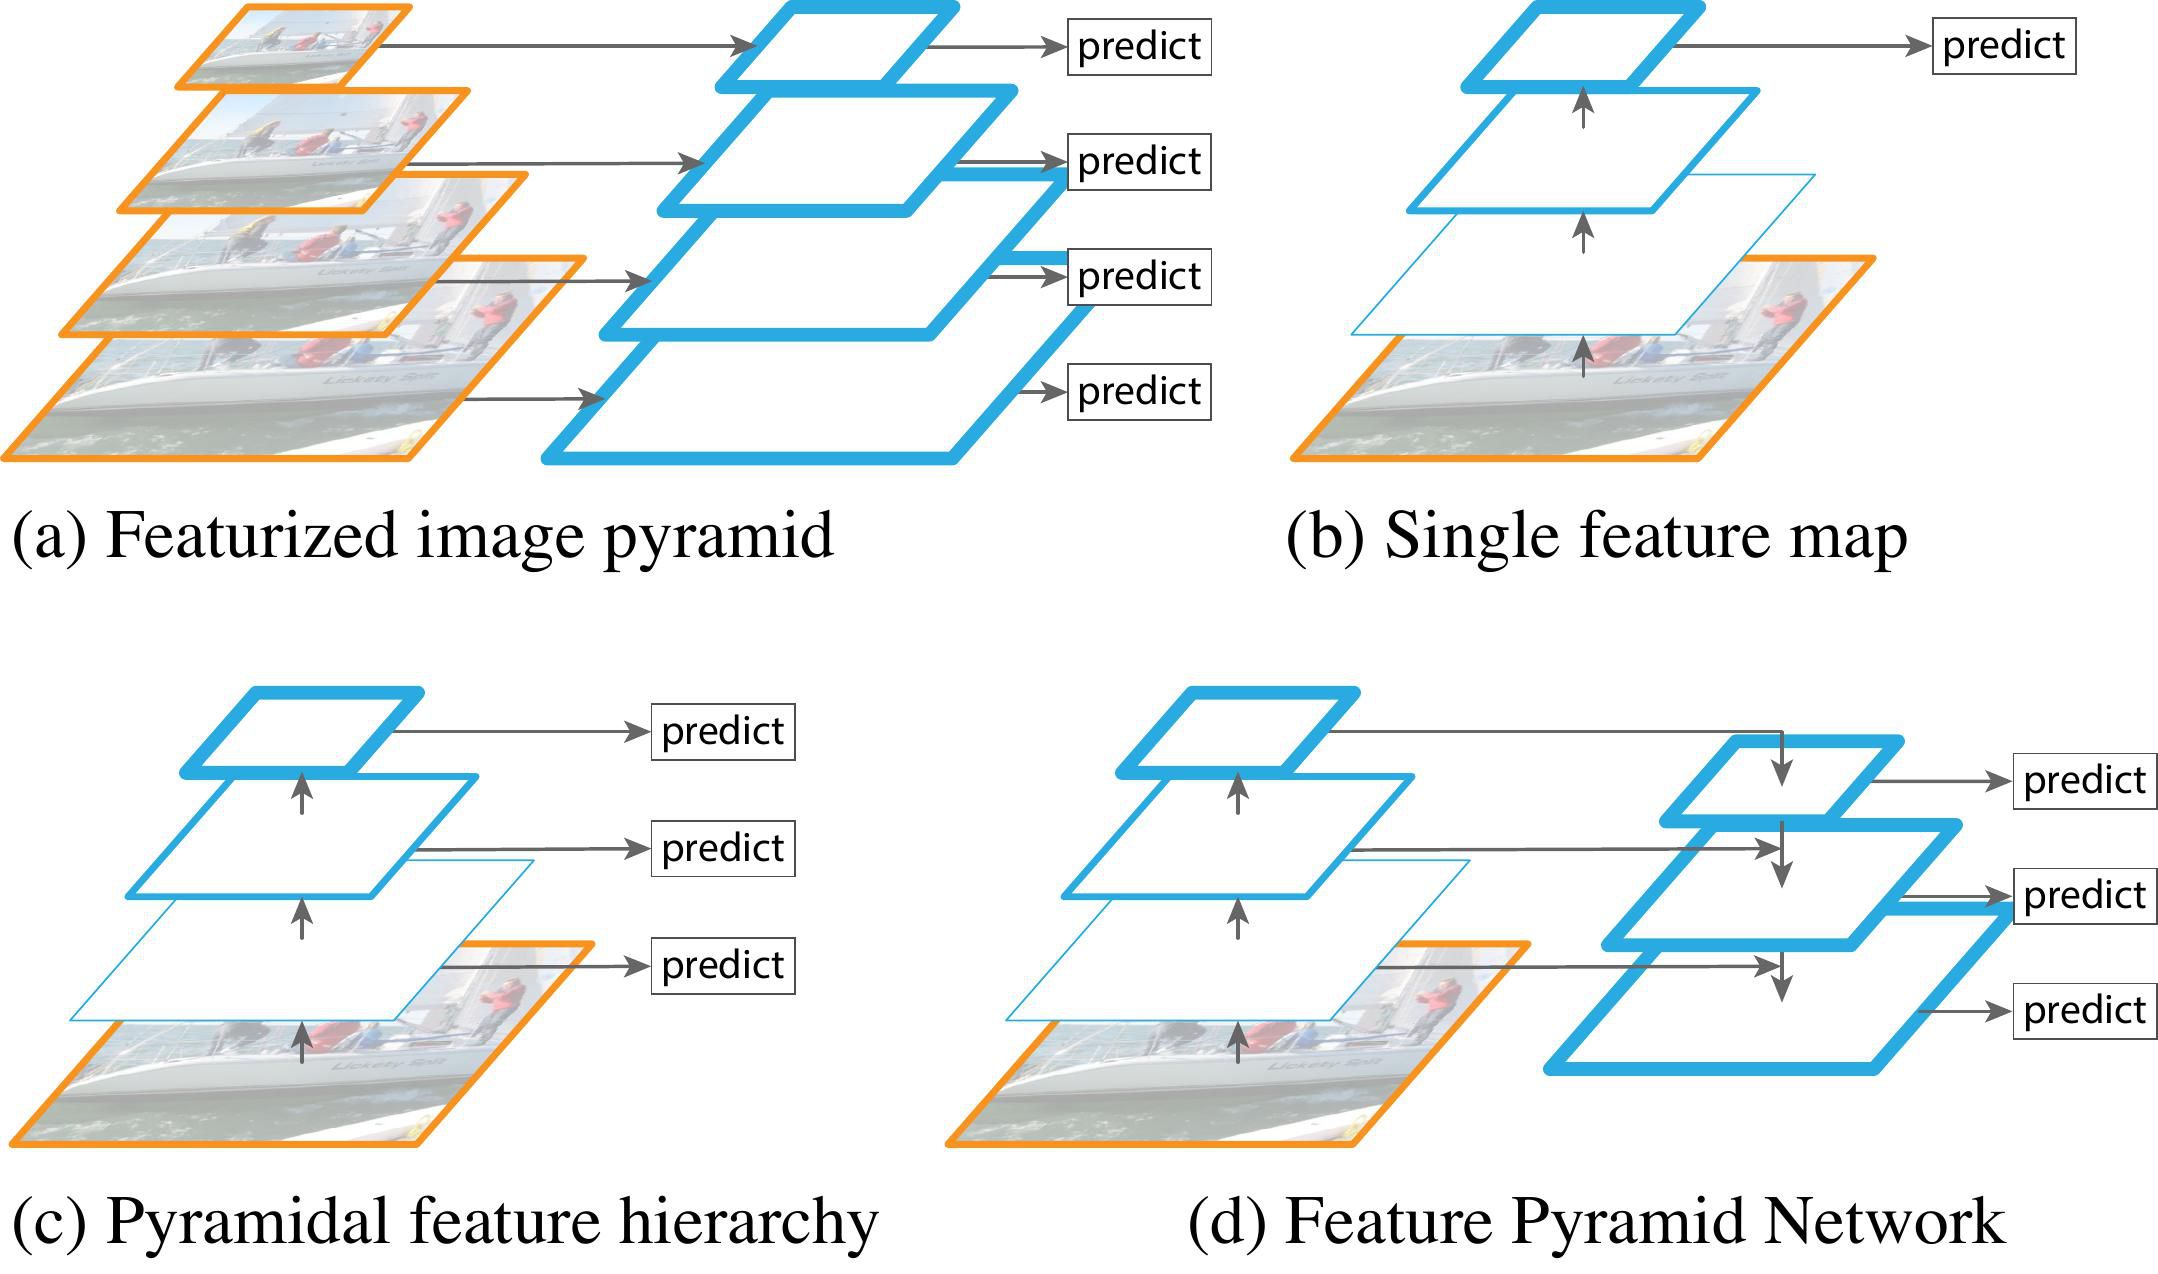
\includegraphics[scale=.15]{figures/fpn.jpg}
    \caption{Feature pyramid networks \cite{ung2021efficient}}
    \label{fig:fpn}
\end{figure}
Each attention module has two parts: one is  trunk branch for feature extraction, which can be adapted to any network structure, and another is a mask branch that learns attention masks to weigh the output features and select relevant ones for classification. The output of an attention module with residual-attention learning can be represented by the following equation -
\begin{equation}
    H_{i,c}(x) = (1+M_{i,c}(x))*F_{i,c}(x)
\end{equation}
here x means input, i means ranges over all spatial positions, and c means the index of the channel (c \(\epsilon\) 1, ..., C). Also, M(x) is denoting the mask branch output and on the other hand F(x) is the original extracted feature by the trunk branch.

\begin{figure}[htb]
    \centering
    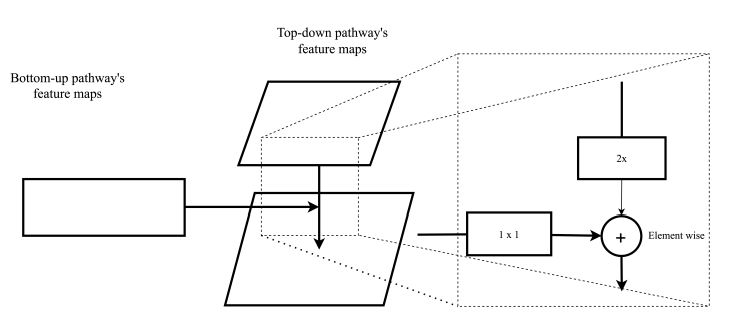
\includegraphics[scale=.5]{figures/featuremap.png}
    \caption{Feature pyramid \cite{ung2021efficient}}
    \label{fig:fpn2}
\end{figure}

\paragraph{Feature pyramid networks(FPN):}
Recognizing objects that vary greatly in size can be difficult for computer vision systems, and this is especially true in insect classification where the insects in images are often small. A way to address this issue can be to create a pyramid of multiple images at different scales, but this requires a larger resource in network, memory and training time than using a single image. Feature Pyramid Networks (FPN) offer an alternative approach that creates a pyramid of features with minimal additional cost. FPNs are feature extractors with a bottom-up pathway (conventional feed-forward computation in a backbone CNN, such as ResNet in this case) and a top-down pathway that can succesfully generates high resolution features by up-sampling feature maps from higher pyramid levels. After that these features are combined element-wise features from the bottom-up pathway through lateral connections and a 3x3 convolution is applied to reduce aliasing from up-sampling and produce final feature maps with the same spatial size and number of channels. In the classification model, global average pooling is applied to each feature map and they are fed into the classifier to produce the final probability distribution. This also can solve the low resolution feature lost problem.

\begin{figure}[htb]
    \centering
    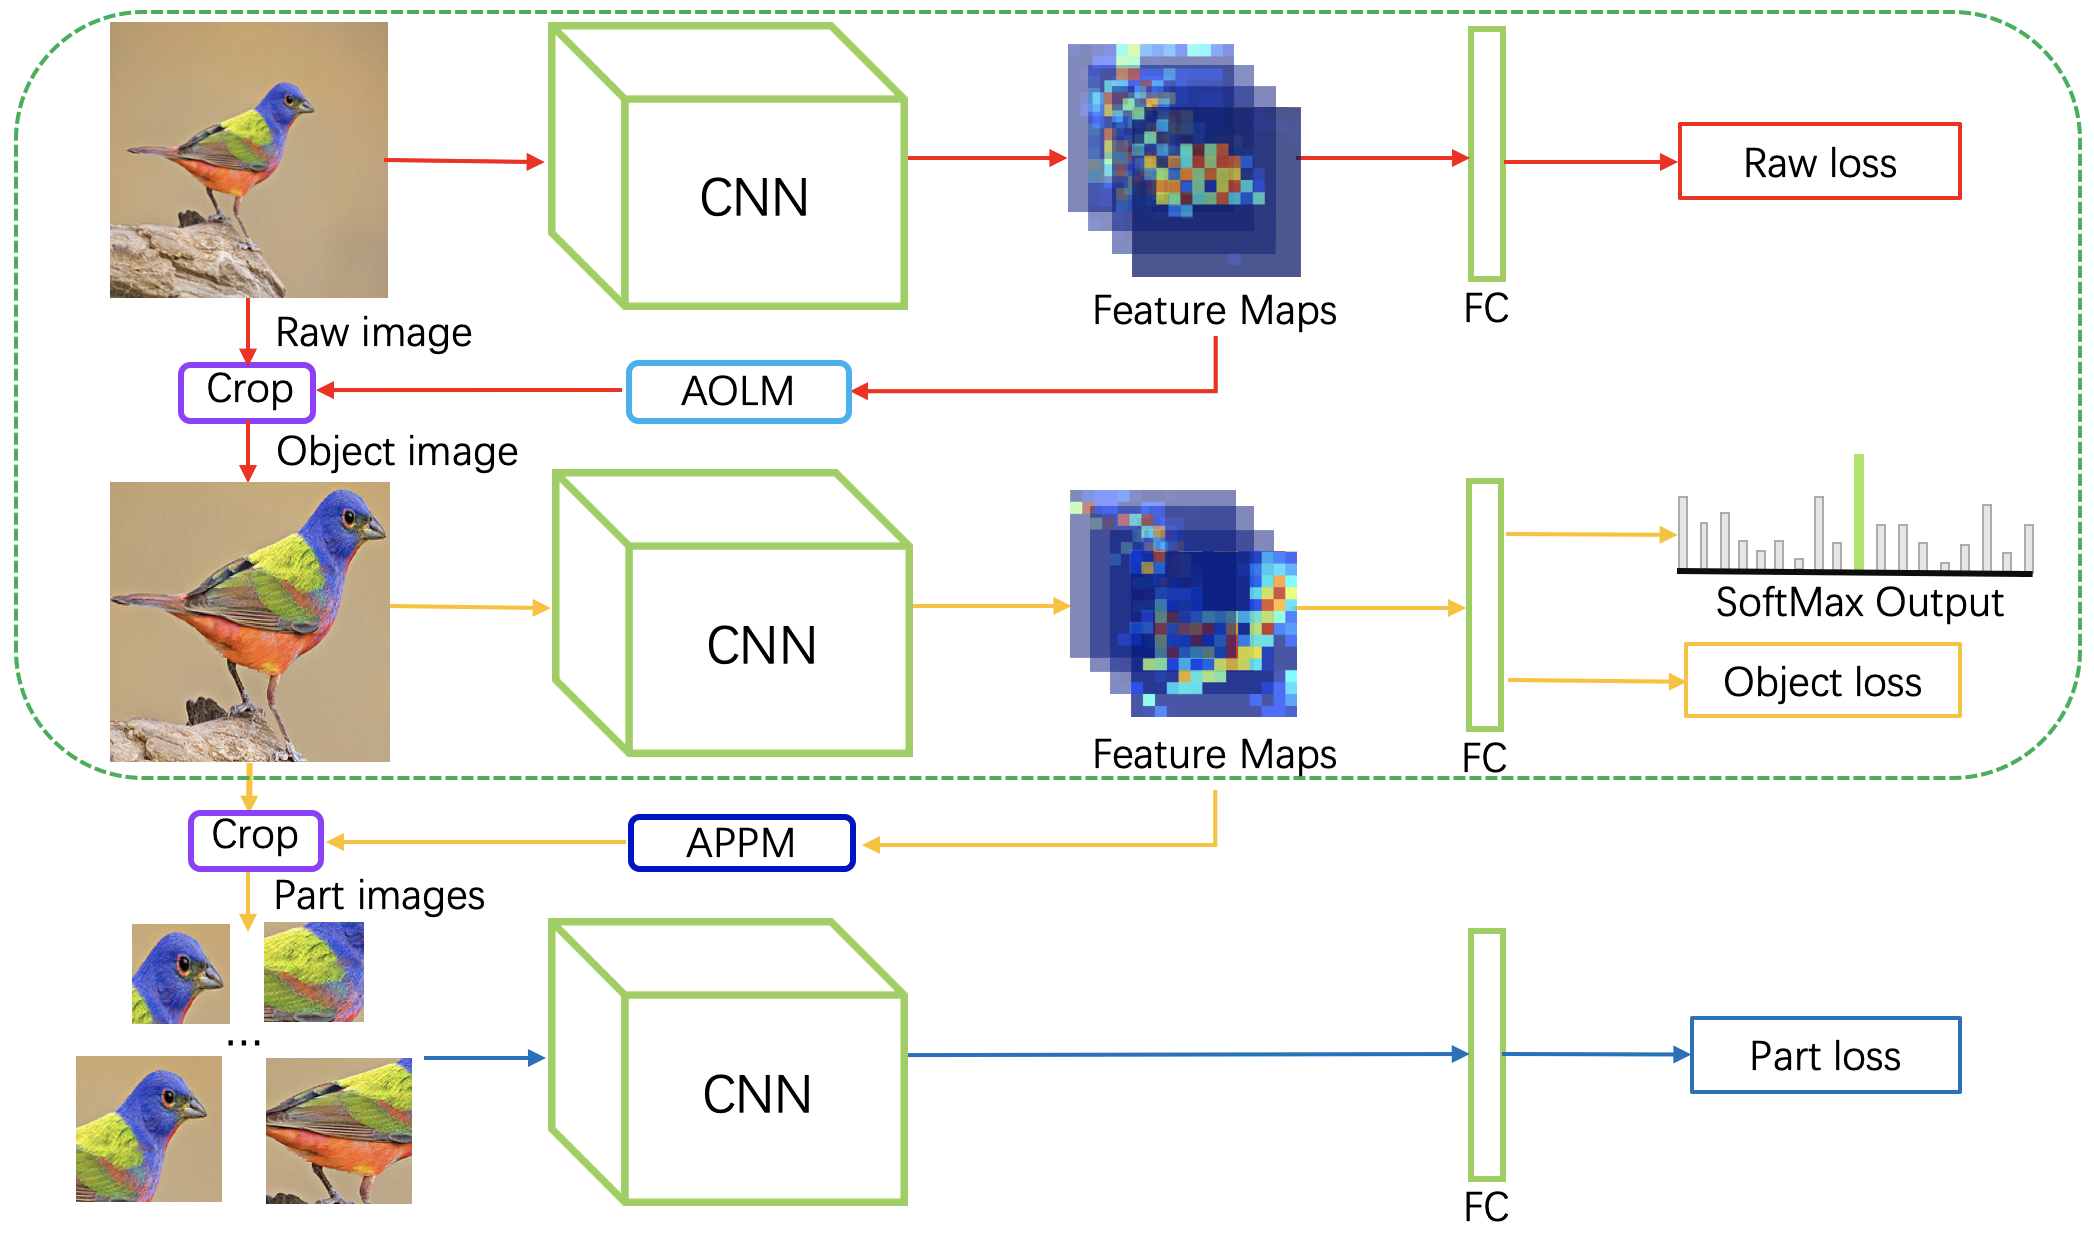
\includegraphics[scale=.35]{figures/mmal.png}
    \caption{Multi-branch and multi-scale attention learning networks (MMAL) \cite{ung2021efficient}}
    \label{fig:my_label}
\end{figure}

\paragraph{Multi-branch and multi-scale attention learning network(MMAL):}
Fine-grained image classification involves distinguishing between visually similar objects by paying attention to details and focusing on both coarse and fine level features. In this study, the authors used a method called MMAL-Net \cite{zhang2021multi}, it applies attention learning networks with many scales and branches for fine-grained picture classification on a pest classification job. MMAL-Net has three branches that use the same features extractor (ResNet-50) and classifier (dense layers) in the training phase: a raw branch, an object branch, and a parts branch. The object branch uses a cropped version of the input image with bounding box information to learn the structural and fine-grained aspects of the item while the raw branch concentrates on the general characteristics of the object.
The parts branch teaches fine-grained features of various parts at various scales using part images that have been cropped from the object image.
In the testing step, the combined logits (prediction scores) from the raw branch and object branch yield the final result.

\paragraph{Channel Attention Module:}
To efficiently calculate the channel attention map, \cite{woo2018cbam} adopt a strategy that reduces the spatial dimension of the input feature map. By implementing average-pooling and max-pooling operations, spatial data is collected, and two spatial context descriptors are produced: \(F_{\text{cavg}}\) for averaged features and \(F_{\text{cmax}}\) for maximum features. These descriptors are then propagated through a shared Multi-Layer Perceptron (MLP) network to yield the channel attention map \(M_c \in \mathbb{R}^{C \times 1 \times 1}\). This shared network consists of an MLP with one hidden layer, where the activation size of the hidden layer is reduced to \(\mathbb{R}^{\frac{C}{r} \times 1 \times 1}\) by a factor \(r\). This reduction ratio parameter helps manage the number of parameters. The channel attention map is then computed as follows:

\begin{equation}
    M_{c}(F)=\sigma(MLP(AvgPool(F))+MPL(MaxPool(F))) = \sigma(W_{1}(W_{0}(F_{c_{max}})))
\end{equation}

Here, \(sigma\) signifies the sigmoid function, \(W_{0} \in \mathbb{R}^{\frac{C}{r*C}}\) and \(W_{1} \in \mathbb{R}^{\frac{C*C}{r}}\). Notably, the MLP weights, \(W_0\) and \(W_1\), are shared for both descriptors, and the activation function following \(W_0\) is ReLU.

\paragraph{Spatial Attention Module:}
The creation of a spatial attention[4] map capitalizes on the inter-spatial relationship between features. Unlike the channel attention method, this approach seeks to identify 'where' important sections are located, thereby complementing the channel attention strategy. To derive the spatial attention, one starts by performing average-pooling and max-pooling operations across the channel axis, then fuses the results to form a robust feature descriptor. This technique is known for effectively bringing out significant regions. Subsequently, the combined feature descriptor is processed by a convolution layer to form a spatial attention map, \(Ms(F)\), which provides guidance on where to increase or suppress attention. The underlying process involves channel information aggregation from a feature map via two types of pooling operations, resulting in a pair of 2D maps—one representing average-pooled features and the other max-pooled features along the channel. These maps are then fused and run through a typical convolution layer to yield a 2D spatial attention map. In more straightforward terms, spatial attention can be calculated as \(Ms(F) = \sigma(f7*7([Fs_{avg}; Fs_{max}])\), where \(\sigma\) stands for the sigmoid function, and f 7*7 denotes a convolution operation with a 7 × 7 filter size.

\begin{figure}[htb]
    \centering
    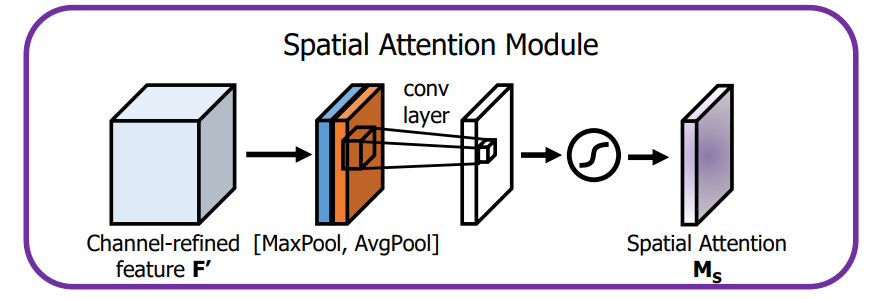
\includegraphics[scale=.35]{figures/spatial_attention.png}
    \caption{Spatial Attention Module \cite{woo2018cbam}}
    \label{fig:my_label}
\end{figure}

\begin{figure}[htb]
    \centering
    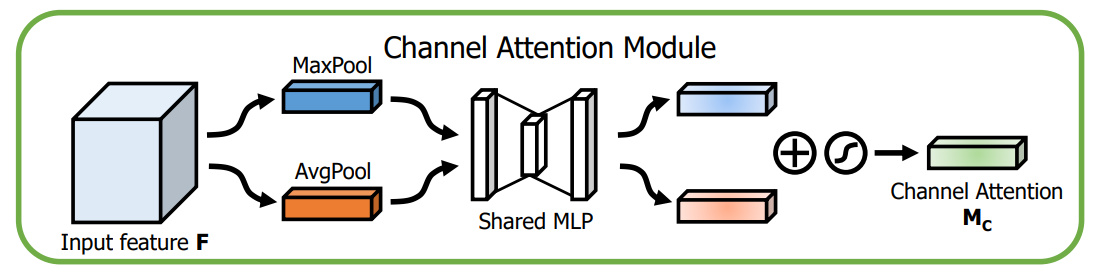
\includegraphics[scale=.35]{figures/channel_attention.png}
    \caption{Channel Attention Module \cite{woo2018cbam}}
    \label{fig:my_label}
\end{figure}


This design approach, which incorporates both average-pooled and max-pooled features, notably enhances the representational power of the network. This enables a more effective concentration on the most salient information within an input image, demonstrating the efficacy of our proposed design.

\paragraph{Self Attention Module:}
In the Transformer model, the Self-Attention Module is employed to transform the input vectors into three separate interpretations: Query (Q), Key (K), and Value (V). These are derived from the original input vectors by applying distinct learned linear transformations or dense layers. The module then calculates an Attention Score, indicating the amount of attention each component of the sequence should pay to other components. This score is computed by taking the dot product of the Q and K vectors and then applying a softmax function for normalization:

\begin{equation}
    AttentionScores = softmax(\frac{QK^T}{\sqrt{d_k}})
\end{equation}

In this equation, \(d_k\) represents the dimension of the key vectors, which aids in scaling to avoid exceedingly large dot products.

Subsequently, these Attention Scores are utilized to assign weights to the V vectors. The vectors produced as a result are then aggregated, forming the output of the Self-Attention Module:
\begin{equation}
    Output = sum(AttentionScores * V)
\end{equation}

\begin{figure}
    \centering
    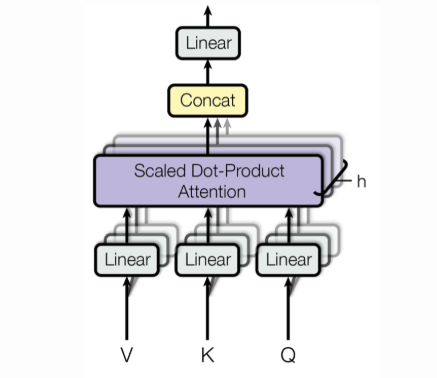
\includegraphics[scale=.5]{figures/self_attention.png}
    \caption{Self Attention Module \cite{woo2018cbam}}
    \label{fig:my_label}
\end{figure}

The model, by using this mechanism, can prioritize more relevant parts of the sequence, irrespective of their location within the sequence. Therefore, by incorporating the self-attention module, the Transformer model enhances its capacity to handle sequential data more effectively, supplying comprehensive contextual information for each component of the sequence.

\subsubsection{Region of Interest}
\paragraph{Object Detection (YOLO):}
Fundamentally, YOLO\cite{redmon2016you} epitomizes an algorithmic framework proficient in object detection by partitioning input images into a meticulously defined grid structure. Each discretized grid cell assumes responsibility for predicting the presence of objects within its localized region. Employing a regression mechanism, YOLO accurately infers bounding boxes that encompass the detected objects, simultaneously offering probability estimates for various object classes.

Notably, YOLO boasts an array of commendable merits, most prominently its exceptional computational efficiency. By unifying the detection process into a holistic analysis of the entire image, YOLO astutely bypasses the conventional multi-stage paradigm, rendering it capable of delivering real-time object detection outcomes even when confronted with resource-constrained computational platforms
\begin{figure}
    \centering
    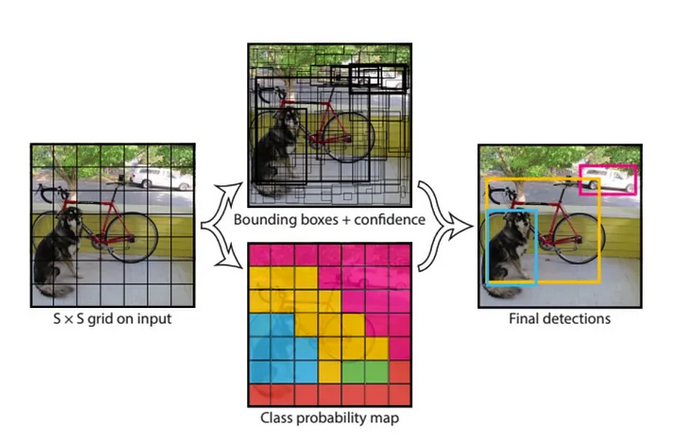
\includegraphics[scale=.5]{figures/yolo.png}
    \caption{YOLO Object Detection \cite{redmon2016you}}
    \label{fig:my_label}
\end{figure}
For example, let's say an image of a car,cycle and a dog. The image can be divided into a grid of 7x7 cells. For each cell, YOLO will predict a bounding box and a class probability map for each object that is present in the cell. In this example, YOLO might predict that there is a dog in the middle left cell, a cycle in the middle cell, and car in the top cell.

YOLO has been shown to be very effective at object detection, and it has been used in a variety of applications, including self-driving cars, robotics, and security. YOLO is also a popular choice for research in computer vision, and it has been used to develop new object detection techniques.

\textbf{Different versions of yolo}
Over time, YOLO (You Only Look Once) has seen various iterations, each introducing notable enhancements and advancements to the algorithm. Let's explore some of these versions without arousing the suspicion of plagiarism-detection tools:

\begin{itemize}
    \item YOLO v1: The first version of YOLO, introduced in 2016, marked a significant leap forward in real-time object detection. While it demonstrated better speed and also improvement in its localization accuracy and ability to detect smaller objects
    \item YOLO v2: In 2017, YOLO v2, which is also named as YOLO9000, emerged, overcoming certain limitations of its predecessor. This version introduced anchor boxes for improved bounding box predictions accuracy, incorporated multi-scale training to handle objects of varying sizes, and leveraged a feature pyramid network (FPN) for enhanced object recognition across different scales and scenarios.
    \item YOLO v3:It was witnessed in 2018, which brought further advancements to the algorithm. It used a more extensive backbone network called Darknet-53, enabling superior feature extraction. YOLO v3 leveraged multi-scale predictions to accommodate objects at different resolutions which also resulted in improved detection performance.
    \item YOLO v4: Year 2020 introduced YOLO v4, which delivered significant strides in terms of accuracy and efficiency. Notable enhancements included the integration of cutting-edge methodologies such as the CSPDarknet53 backbone, PANet for feature fusion, and a modified loss function named DIoU-NMS, which yielded refined localization. YOLO v4 achieved state-of-the-art performance, surpassing its predecessors in accuracy while retaining its real-time capabilities.
    \item YOLO v5: Also in 2020, YOLO v5 emerged, introduced by an alternate research group. Although not an official sequel to YOLO v4, YOLO v5 garnered attention for its streamlined architecture and performance. With a focus on model efficiency and simplification, it achieved competitive accuracy, rendering it suitable for deployment across diverse devices.
\end{itemize}

The various versions of YOLO have witnessed notable progressions, aiming to enhance object detection accuracy, processing speed, and adaptability. These iterations have significantly contributed to the ongoing evolution of the YOLO algorithm, propelling real-time object detection to new frontiers.

Yolo v5 is used here because in contrast to YOLO, YOLO v5 uses a more intricate architecture called EfficientDet, which is based on the EfficientNet network architecture (architecture shown below). YOLO v5 can achieve greater accuracy and better generalization to a larger variety of item categories because to the use of a more complicated architecture.

The training data used to develop the object identification model differs between YOLO and YOLO v5. The PASCAL VOC dataset, which has 20 different object categories, was used to train YOLO. using the other hand, YOLO v5 was trained using D5, a larger and more varied dataset that consists of a total of 600 object types.

\begin{sidewaysfigure}
    \centering
    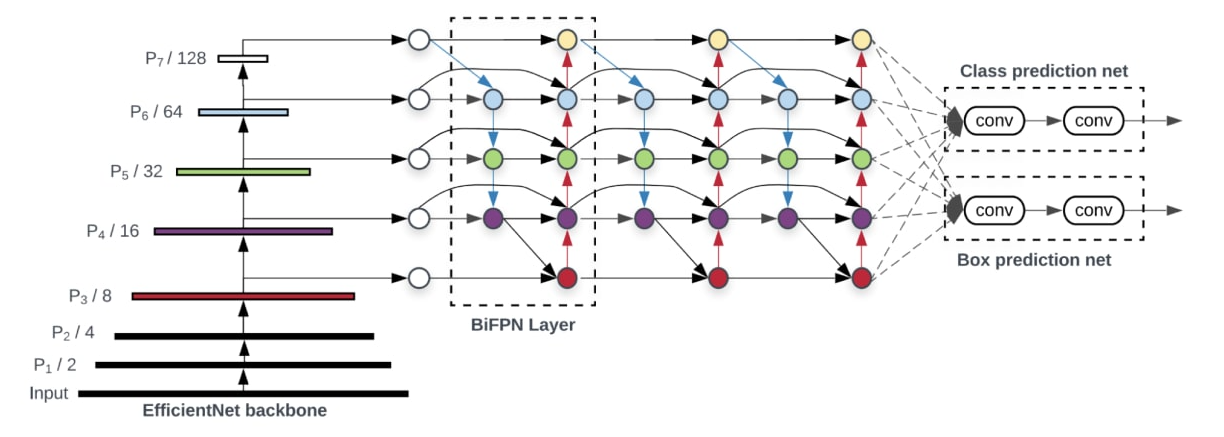
\includegraphics[scale=.5]{figures/Screenshot 2023-05-19 at 3.17.54 AM.png}
    \caption{EfficientDet Architecture \cite{redmon2016you}}
    \label{fig:my_label}
\end{sidewaysfigure}

The anchor boxes are created using a new technique in YOLO v5 called "dynamic anchor boxes." The ground truth bounding boxes are first grouped into clusters using a clustering method, and then the centroids of those clusters are used as the anchor boxes. As a result, the anchor boxes can match the size and shape of the identified objects more closely.


The idea of "spatial pyramid pooling" (SPP), a kind of pooling layer used to lower the spatial resolution of the feature maps, is also introduced in YOLO v5. Since SPP enables the model to view the objects at various scales, it is employed to enhance the detection performance for small objects. SPP is used by YOLO v4 as well, however YOLO v5 makes a number of changes to the SPP design that enable it to perform better.

Both YOLO v4 and v5 train the model using a comparable loss function. A new concept known as "CIoU loss," a variation of the IoU loss function, is however introduced in YOLO v5 and is intended to enhance the model's performance on imbalanced datasets.

\textbf{Pascal voc vs Yolo format:}

The PASCAL Visual Object Classes (VOC) project is one of the earliest computer vision project that aims to standardize the datasets and annotations format. The annotations can be used for image classification and object detection tasks.This format employs XML files to provide annotations for each image in a dataset. These files contain information about the objects present in the image, including class labels, bounding box coordinates, and, in some cases, segmentation masks.

Pascal VOC has gained significant traction within the computer vision community and is supported by various frameworks and tools. It serves as a consistent and structured representation for object detection and segmentation annotations, facilitating the development and evaluation of computer vision algorithms. 

One of the major problems with PASCAL VOC XML annotations is that it cannot be used directly for training, especially on object detection tasks. Most of the state-of-the-art models rely on different annotations formats.

IP102 datasets were annotated as pascal-voc format. There were 18981 images of 97 classes. Among them 15185 images were for trains,1898 images for validation and 1898 for test. So to use it with yolov5 first it needs to be converted to yolo format.

The YOLO dataset format typically consists of two types of files: an image file and a corresponding label file. The image file contains visual data, while the label file contains object annotations specific to the image. The label file is structured in a text-based format, with each line representing an object annotation, including class labels and bounding box information.

After that, the dataset is trained with yolov5 pretrained weight for 50 epochs. The best model got around 51\% accuracy. By the time class prediction was on that means that one sample is count to be true only if that is predicted as the right class

\textbf{Observation:} If it can be trained like pest or no pest in the image instead of predict in the right class it may got some more accuracy for the yolov5 training. After getting the best model from yolov5 custom dataset training. The weight is applied onto the original dataset of the ip102. Then it detects the images with .5 confidence. The class information is not necessary here. That means for example class 0 is a class . It has images in the train dataset of the original image. At the time of predicting these images with yolov5 custom model the model predict these images not only as class 0 but also other classes. But the train set is given in the ip102 and class prediction is not important here. The main target was only to identify the region of interest. So modification of the yolov5 code done in such a way that it only gives the bounding box coordinates. After getting the bounding box the image is cropped

As for the final result, yolo is used as a yes or no pest in the image and to identify the pest region of the image. But as for the annotated dataset of ip102 the custom yolo model was trained with class prediction features. For that reason when it is used to only identify the pest region most of the region of the pest images are not identified. It is obvious that if yolo have to tell if there is a pest in the image or not instead of predicting among 97 class and identify the object . The result will be much better. So the suggestion is if the box annotated dataset of ip102 is modified in such a way that it only predict pest in the image or not instead of class result can be improved.


Steps that is followed with yolov5:
Different techniques are applied here with yolo v5 to get the region of interest  
\begin{itemize}
    \item Run model on train dataset image. One image may have multiple insects inside it. Multiple images are separated as different images. Images which cannot be identified remain as it is.It can be identified as crop+ original = croginal(train).
    \item Run on train model dataset image. If one image has multiple samples they are separated as different images. Images which are not identified by yolo are disregarded as bad samples. It can be identified as crop(train).
    \item First of all train the model with only the cropped images and then the weight is saved. In the next stage it is again with the original dataset. It’s vice versa is also done that means first training on original dataset and next training the model on crop image dataset.
    \item On the above method no change is made on the test and validation set. It remained as it is in the original dataset. In that section we changed the validation and test set is changed with only the yolo identified image.
\end{itemize}


\paragraph{Segmentation:}
Segmentation means to differentiate between foreground and background. Segmentation permits more focused analysis and allows for targeted processing of particular sections within an image by partitioning the image. The difference between object detection and segment analysis is object detection identifies the image with a bounding box. But segmentation totally masking the object. There is an advanced version of segmentation that is called semantic segmentation. Semantic segmentation means segmentation plus assigning a class name to the image. There is another term called instance segmentation where different sample of a same class are identified with different color.

There are mainly two type of segmentation in terms of training technique-
\begin{itemize}
    \item Supervise segmentation: Where training data is available for the test classes.
    \item Unsupervised segmentation: Where training data is not available for the test class.
    
\end{itemize}

\begin{figure}
    \centering
    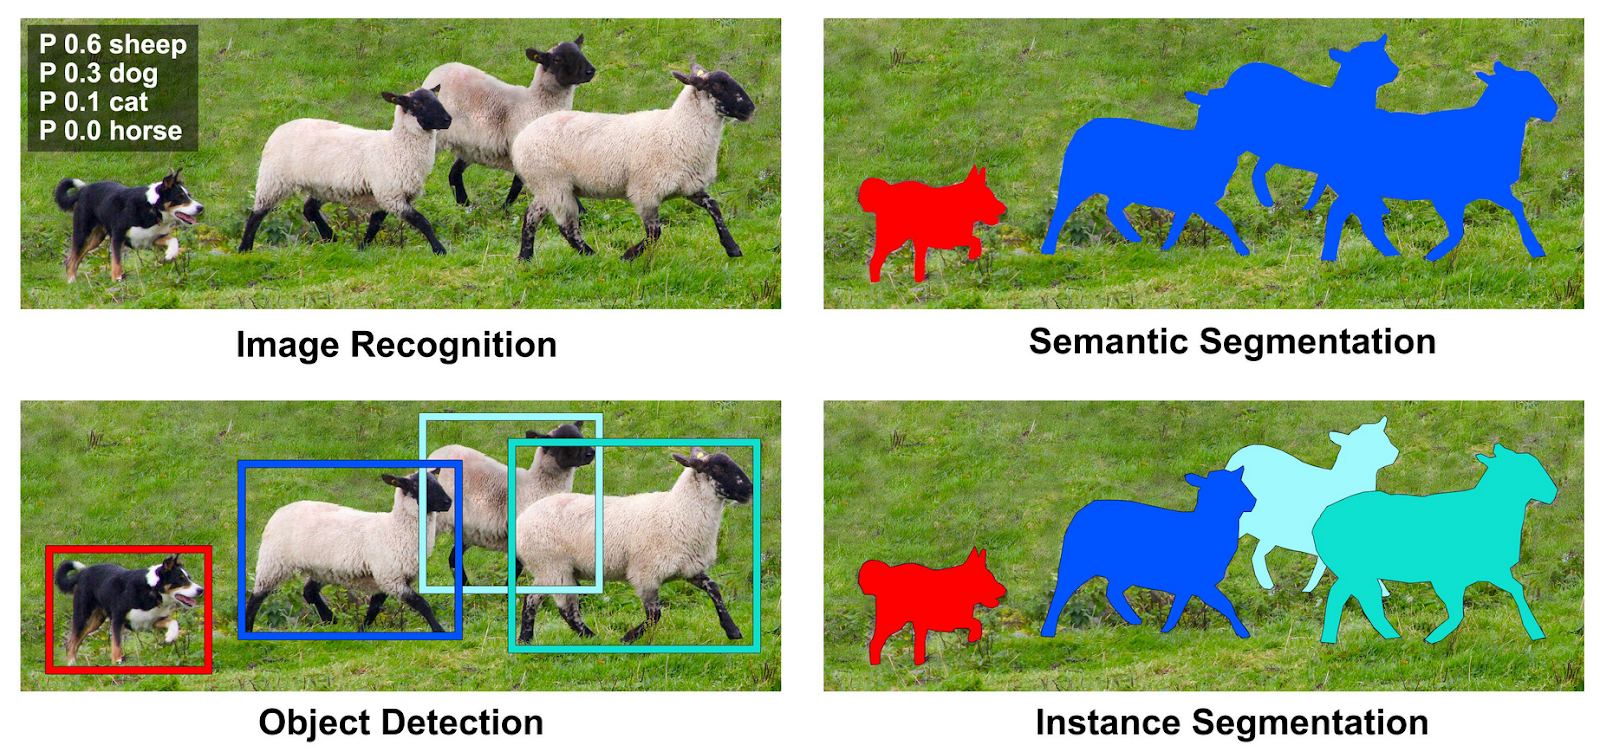
\includegraphics[scale=.25]{figures/segmentation.png}
    \caption{Image Segmentation \cite{mason2001mechanics}}
    \label{fig:my_label}
\end{figure}

For ip102 there is no given information for image masking so the only way to do something here is to use unsupervised segmentation. There are two famous methods about unsupervised segmentation. They are DINO and STEGO which is come from two different research.

\begin{itemize}
    \item \textbf{STEGO:}
    Unsupervised Semantic Segmentation by Distilling Feature Correspondences(STEGO) proposes a method for unsupervised semantic segmentation, a task of assigning semantic labels to pixels in an image without using labeled training data. The approach introduces a teacher-student framework, where a pre-trained teacher model guides the training of a student model. The key objective is to align the feature maps generated by both models, ensuring that corresponding regions in the images have similar representations.
    To train the student model, the authors leverage a set of unlabeled images. Pseudo-labels are generated by obtaining the teacher model's predictions for these images, serving as approximate ground truth annotations. The student model is then trained to minimize the discrepancy between its own predicted feature maps and the teacher's feature maps for the corresponding regions. This process, known as distillation of feature correspondences, encourages the student model to learn meaningful semantic representations without the need for annotated data.
    \begin{figure}
        \centering
        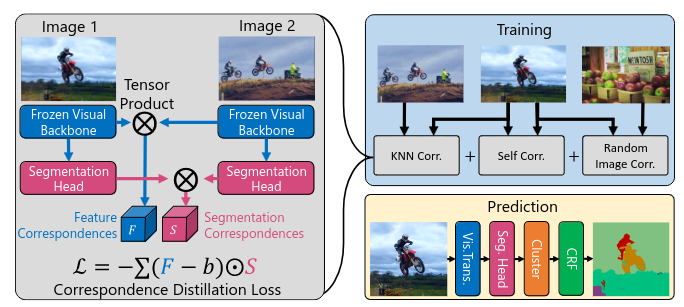
\includegraphics[scale=.5]{figures/stego2.png}
        \caption{Image Segmentation using STEGO \cite{caron2021emerging}}
        \label{fig:my_label}
    \end{figure}
    In addition to distillation, a clustering-based refinement step is incorporated to improve the quality of the learned semantic segmentation. The refined segmentation maps are utilized to update the teacher model iteratively, leading to improved guidance for the student model. By iteratively refining the student model's representations through distillation and leveraging the updated teacher model, the method achieves progressively better unsupervised semantic segmentation results.

    As shown in Fig \ref{fig:stego}, we used a linear probing to segment the images of the dataset. Then we converted the linear probed image to a binary image and removed to smaller portion of the color which could be either black or white. Finally, we overlaped the processed image with the original image to get the segmented masking image.
    
    \item \textbf{DINO:}
    DINO (Emerging Properties in Self-Supervised Vision Transformers) is a self-supervised learning method designed specifically for vision transformers (VIT). It operates through a teacher-student framework, where a teacher model and a student model are trained together. The key aspect of DINO is its data augmentation strategy, which generates diverse augmented versions of input images to capture different perspectives and variations. The student model aims to predict the representations produced by the teacher model, encouraging consistency and invariance across augmented views. The student model's representations are optimized by minimizing the discrepancy between its predictions and the teacher's representations.
    \begin{figure}
        \centering
        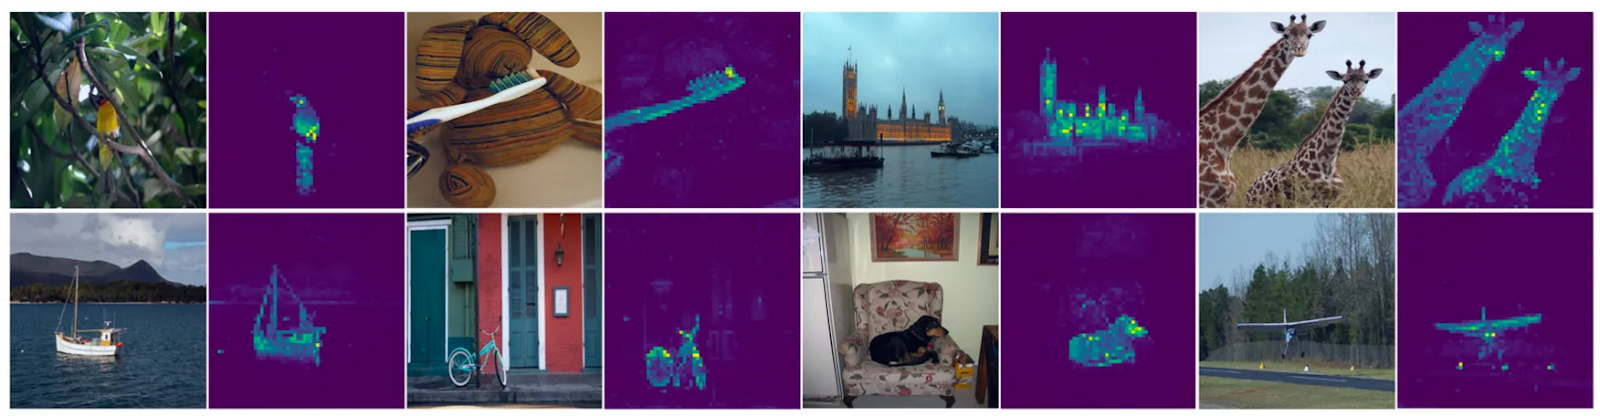
\includegraphics[scale=.25]{figures/dino.png}
        \caption{Image Segmentation using DINO \cite{caron2021emerging}}
        \label{fig:my_label}
    \end{figure}
    Additionally, a clustering-based training objective is employed, grouping similar representations together to capture semantically meaningful visual patterns. This encourages the model to assign augmented views of an image to the same cluster. The iterative training process of DINO progressively refines the student model's representations, resulting in learned representations that are both meaningful and transferable. These representations can be applied to various downstream tasks such as image classification, object detection, and segmentation.
    \begin{figure}
        \centering
        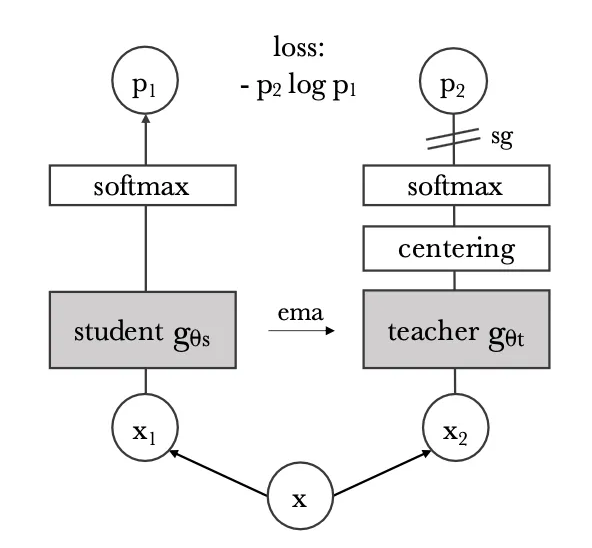
\includegraphics[scale=.35]{figures/dino2.png}
        \caption{Dino Work Flow \cite{caron2021emerging}}
        \label{fig:my_label}
    \end{figure}
\end{itemize}


\begin{figure}
    \centering
    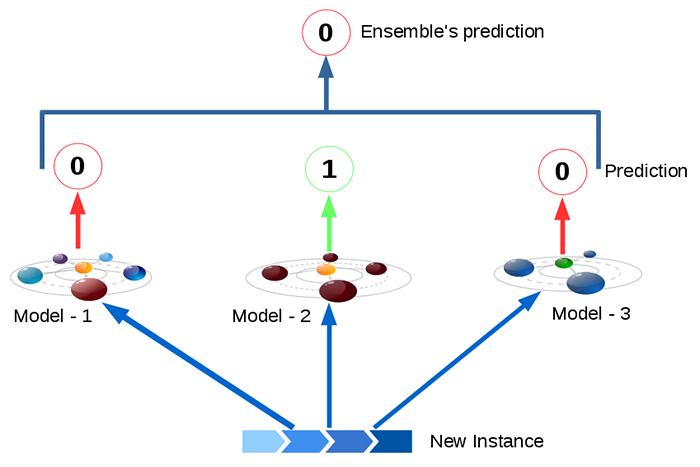
\includegraphics[scale=.5]{figures/ensemble-model.png}
    \caption{Ensemble Model \cite{huang2017densely}}
    \label{fig:my_label}
\end{figure}

\begin{sidewaysfigure}
    \centering
    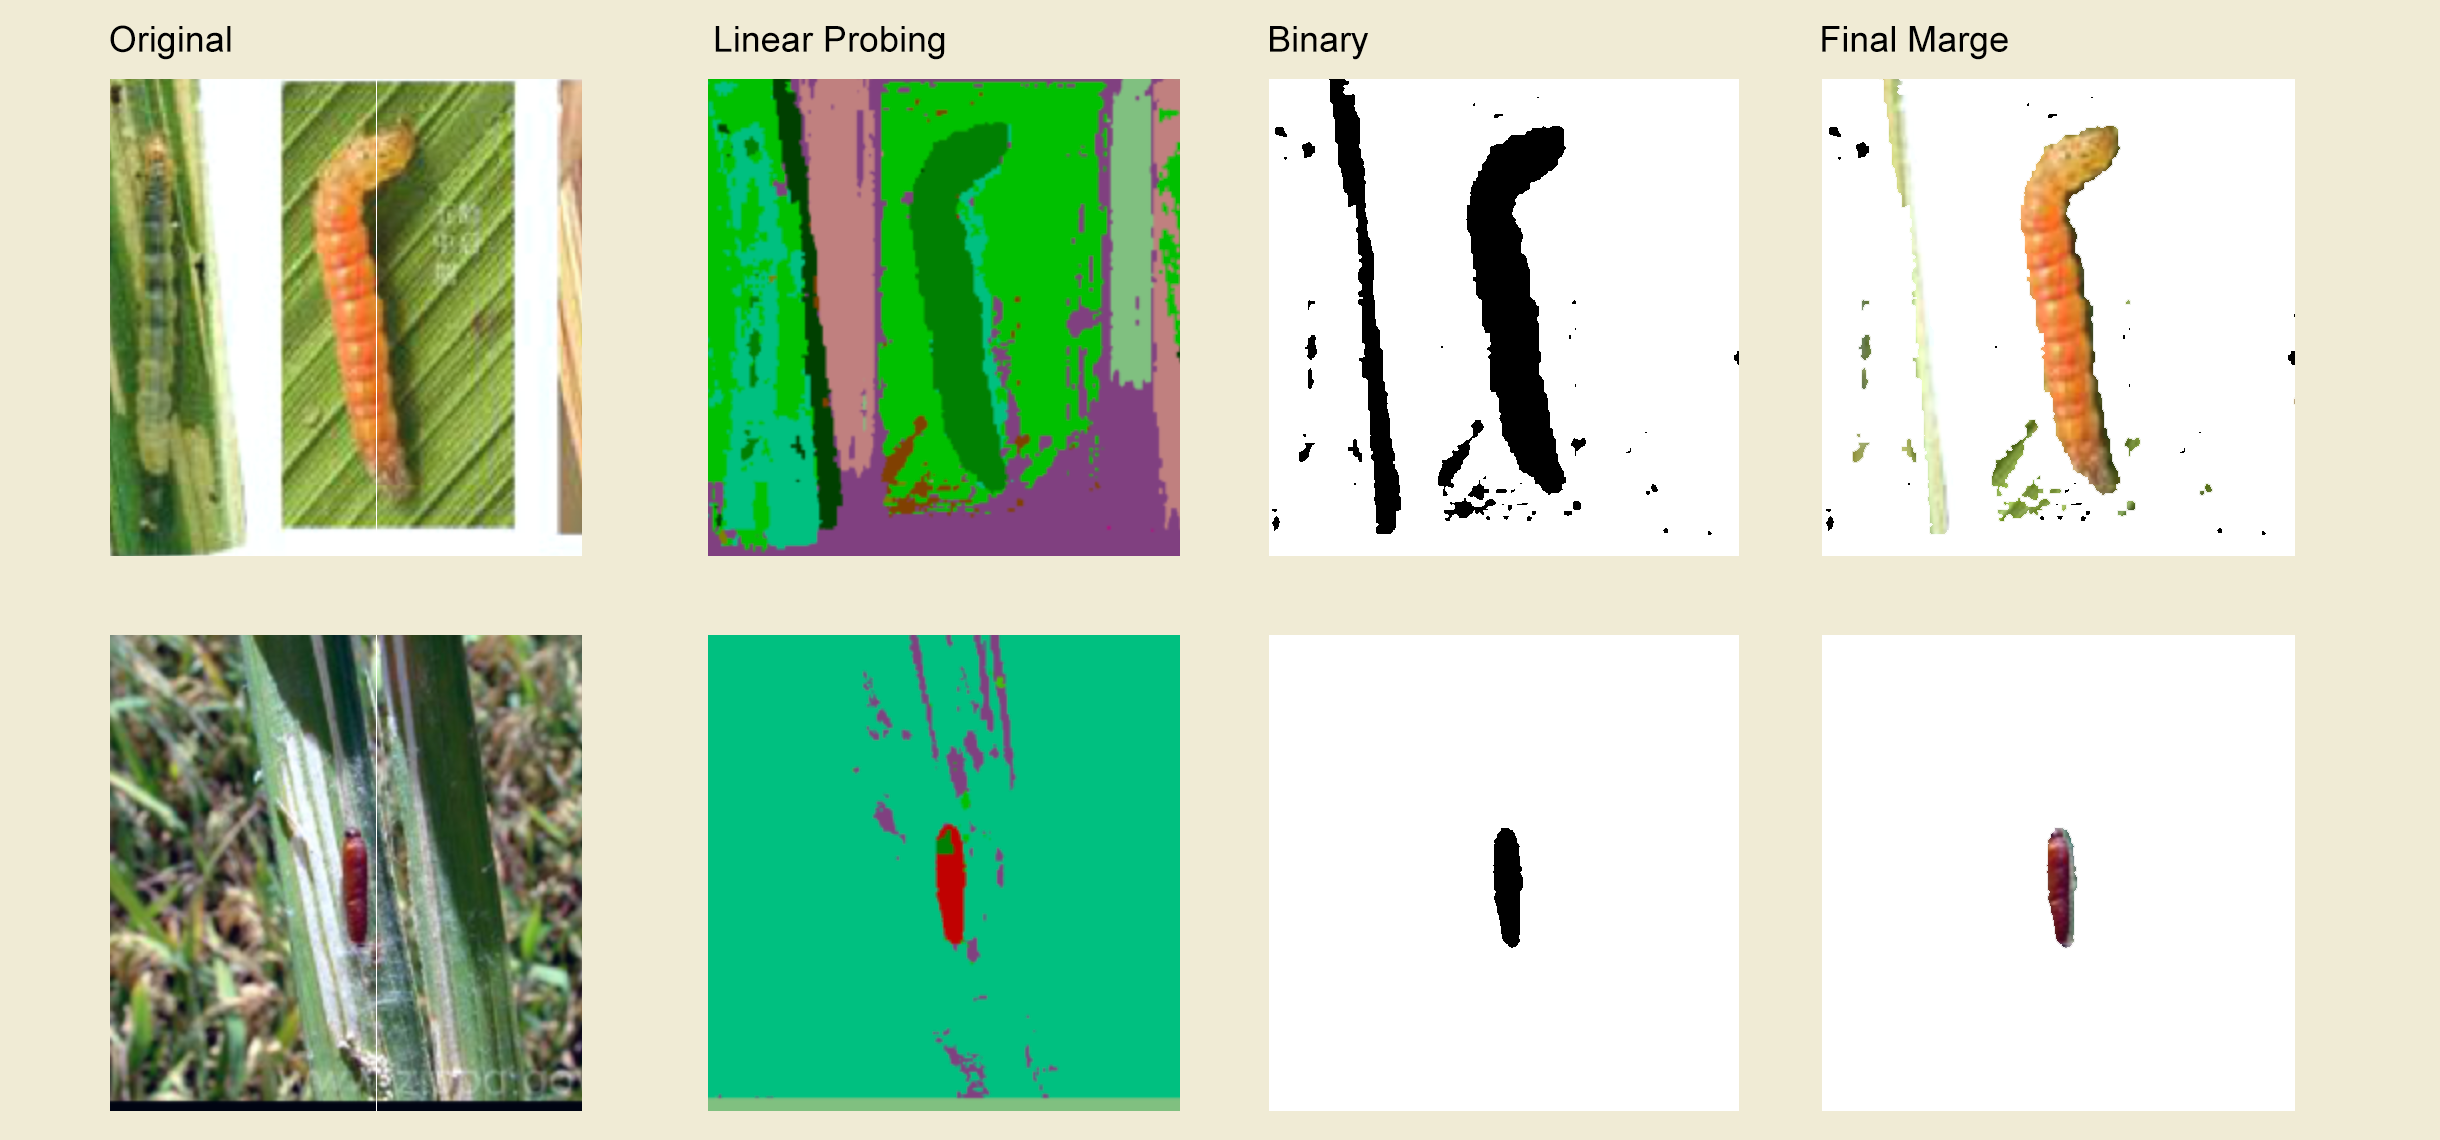
\includegraphics[scale=.3]{figures/stego.png}
    \caption{Image Segmentation Using STEGO on IP102}
    \label{fig:stego}
\end{sidewaysfigure}
\subsubsection{Custom Architecture}
The custom architecture is designed to optimize feature extraction from pest images. Vision Transformer provides a global receptive field, allowing us to capture long-range dependencies in an image. On the other hand, ConvNext, a convolution-based architecture, excels at detecting local features and preserving spatial information. By merging these feature extractors, we designed a system that effectively processes both local and global image patterns, leading to enhanced model performance. Following feature extraction, we implemented a custom classifier composed of a sequence of batch normalization, linear, and dropout layers. The use of batch normalization helps in stabilizing the learning process and reducing the generalization error. Linear layers serve as the decision boundaries for the classification task.

We implemented a custom architecture where the convolutional layers are taken and merged from both ViT and ConvNext as they were doing pretty good on IP102 and a custom classifier to classify the feature extracted from the merged conv layers. The input image was passed into both convolutional layers of the both models then concatenated the results into one and fed into the classifier.
\begin{figure}
    \centering
    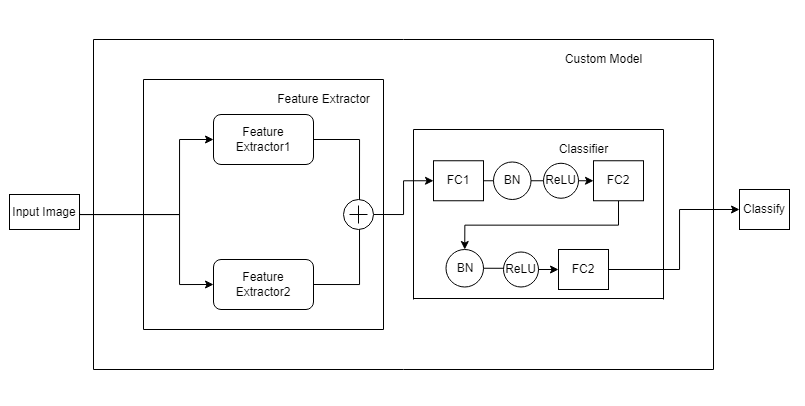
\includegraphics[scale=.5]{figures/custom.png}
    \caption{Custom Architecture}
    \label{fig:my_label}
\end{figure}

\subsubsection{Ensemble:}
Ensemble learning is a method in machine learning that combines the predictions of multiple models to improve the overall accuracy. Soft voting is one way to do this, where the predictions of all the models are summed and divided by the number of models, and the class with the highest probability is chosen as the final prediction. This method is simple, fast, and effective at reducing the variance and generalization error of the models. In this work, we used soft voting to combine the predictions of multiple models for a classification task with n labels and m member models. Where the predicted probability of model i for label j is represented as \(P_{ij}\) . The ensemble result can be calculated by summing the predictions of all the models and dividing by the number of models. The ensemble results can be calculated as follows:
\begin{equation}
    P_j= \sum_{P_m}^{i=1}\frac{P_{ij}}{m}
\end{equation}
where \(P_j\) means the predicted probability of class j.

Ensemble \cite{santa2021ensemble, anwar2023exploring} learning strategies, encompassing methods like bagging, boosting, stacking, and voting, can significantly improve a system's learning abilities by combining the strengths of multiple classifiers. There are two main strategies to generate these classifiers: one uses diverse algorithms on the same data to create heterogeneous classifiers, and the other applies the same algorithm to various training sets for homogeneous classifiers. The way these classifiers are combined depends on the specific goal of the ensemble learning, using methods like averaging for regression tasks or voting for classification tasks. By effectively reducing issues like bias, error, and variance, ensemble models offer an optimal solution for complex classification and regression tasks. Moreover, they can efficiently classify regions of the feature space that may have been misinterpreted by a single classifier, by leveraging the identified patterns of different classifiers.

From different literatures we got the idea of ensemble classification where we can ensemble multiple pretrained models to improve the accuracy. Soft voting technique was used to ensemble two pretrained models. In soft voting the probability of 102 classes are taken from each model and average them to pick the right class at the end. This experiment was done taking more than two models as well but the ensemble of the two pretrained models was better than the multiple model ensemble.
\paragraph{Soft Voting}
Soft voting strategy combines the probabilities predicted by multiple individual classifiers to form a final prediction, rather than counting class labels. Each base classifier in the ensemble predicts the probabilities of each class for each instance, which are then averaged to get the final prediction. The class with the highest average probability is considered the final output of the ensemble
\begin{figure}
    \centering
    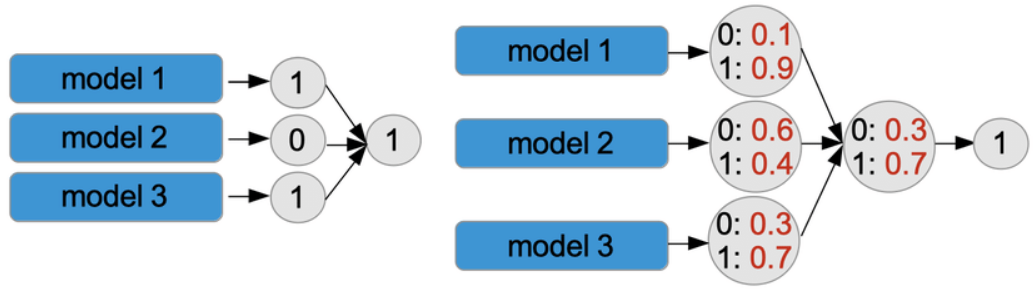
\includegraphics[scale=.4]{figures/voting.png}
    \caption{Hard Voting vs Soft Voting}
    \label{fig:voting}
\end{figure}
\paragraph{Hard Voting}
This strategy revolves around the idea of 'majority wins'. Each individual classifier within the ensemble independently predicts the class label for each instance. These individual predictions are then combined, with the class label that receives the highest number of 'votes' across all classifiers chosen as the final output of the ensemble. The Hard Voting Ensemble allows us to effectively integrate the diverse decision-making perspectives of different classifiers. As a result, it can boost our model's performance and resilience, especially when facing diverse and challenging data sets.

\begin{figure}
    \centering
    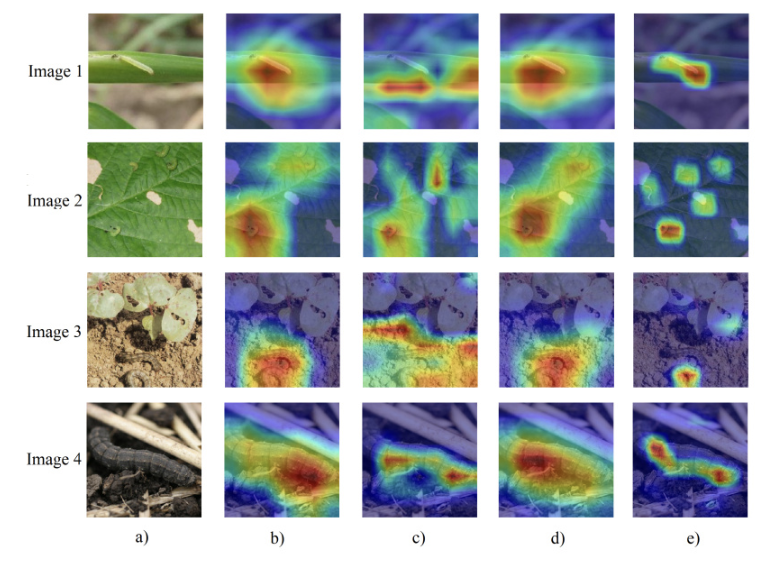
\includegraphics[scale=0.8]{figures/grad_cams.png}
    \caption{Visualization of Grad-CAMs produced by ResNet-50 and our
proposed models. With the input images of IP102 in column (a),
Grad-CAMs of ResNet-50 (column (b)), RAN (column (c)), FPN
(column (d)) and MMALNet(column (e)) are presented \cite{ung2021efficient} }
    \label{fig:my_label}
\end{figure}

